\section{Contexto histórico}
La burbuja del Mississippi sucedió en Francia a principios de 1.700. Tuvo su desarrollo en paralelo a la burbuja de la Compañía de los Mares del Sur de Gran Bretaña, explicada en el capítulo cuatro.
El país se encontraba devastado económicamente por la Guerra de Sucesión Española y por los gastos que realizaba cotidianamente la monarquía. El rey Luis XV tenía cinco años de vida y el país estaba gestionado por el duque regente Felipe II de Orleans. 

La burbuja del Mississippi comenzó en 1.715, cuando el gobierno francés estaba prácticamente en quiebra debido al peso de las deudas contraídas durante la mencionada Guerra de Sucesión. El gobierno no pagó parte de su deuda y tomó medidas prebentibas como la reducción de los pagos de intereses y elevó los impuestos a niveles muy altos. Estas medidas, sirvieron para deprimir la economía francesa y devaluar el valor de su oro y de la moneda de plata con violentas fluctuaciones. 

El gobierno francés, dirigido por un grupo de regentes del rey Luis XV, estaba ansioso por encontrar una solución a los problemas fiscales y económicos de la nación. El duque de Orleans y líder del grupo de regentes, decidió buscar el consejo de su amigo, John Law, quién era un teórico temprano de la economía monetaria.

Law, prometió grandes beneficios procedentes de América del Norte, más concretamente del territorio del Mississippi. Para desgracia de los inversores, las perspectivas de la compañía resultaron ser poco más que promesas vacías, pues contribuyeron a arruinar el mercado de valores de Francia y las finanzas públicas del país.

\section{El sistema de John Law}

John Law provenía de Fife, Escocia, donde nació en una familia acomodada de banqueros y orfebres. Law se convirtió en aprendiz de su padre a los catorce años y estudió las actividades bancarias hasta la muerte de su padre, tres años después. Con veintitrés años, Law viajó a Londres en busca de aventura donde se ganó la vida como jugador gracias a sus habilidades matemáticas. Por ello, se vio envuelto en un duelo donde asesinó a su rival y fue acusado de homicidio y condenado a muerte. Pero John Law estuvo un breve tiempo en prisión antes de escapar a la Europa continental, donde estudió altas finanzas en ciudades como Amsterdam, Venecia y Génova. En 1.705, Law, publicó un trabajo académico en el que manifestó estar en contra del uso de la moneda respaldada por metales preciosos y a favor del \emph{dinero papel} o moneda fiduciaria, afirmando, según recoge Smant (2001), que el uso del dinero papel estimularía el comercio. Debido a estos particulares puntos de vista, Law es a menudo considerado como un economista de estilo keynesiano temprano. 

En 1.716, Law aplicó su teoría monetaria y estableció tres cambios en el mercado financiero Francés. 

En primer lugar, recibió el permiso del gobierno de Francia para fundar un banco, le \emph{Banque Générale}. Este banco tenía depósitos de oro y plata y los intercambiaba por el \emph{dinero papel}. Los billetes emitidos por éste, no eran moneda de curso legal, pero fueron aceptados como tales por la ciudadanía francesa. El banco constituyó sus reservas a través de la emisión de acciones y de los beneficios obtenidos gracias a la gestión de las finanzas del gobierno francés. 

En segundo lugar, a partir del año 1.717, John Law utilizó su influencia, cada vez mayor dentro de la sociedad francesa, para adquirir el monopolio de una de las empresas comerciales más relevantes de Francia: \emph{la Compañía de Mississippi}, a la que él denominó la \emph{Compagnie d'Occident}. Esta empresa dominaba multitud de territorios en América del Norte. Una amplia franja de lo que es Louisiana en la actualidad, hasta Canadá \footnote{Se puede comrpobar en el mapa del Anexo II}. Estos territorios fueron considerados por la sociedad francesa como valiosos por su abundancia de recursos, tales como pieles de castor y metales preciosos. Más tarde, la población francesa descubrió que se trataba de un engaño por parte de John Law. 

En tercer lugar, en julio 1.719, dicha compañía adquirió el derecho de acuñar nuevas monedas. Un mes más tarde adoptó el derecho de cobrar todos los impuestos indirectos franceses y en octubre de 1.719 comenzó a recaudar los impuestos directos. Por último, se puso en marcha una reestructuración de la mayor parte de la deuda nacional, por lo que parte de la deuda pública existente, se intercambiaría por acciones de la Compañía. En ese momento, la Compañía fundada por Law, había absorbido multitud de compañías con las que controlaba tanto el comercio francés como sus finanzas. Por consiguiente, la compañía se renombró como la \emph{Compañía de las Indias}. 

Así, en enero de 1.719, la Compañía de las Indias ofreció acciones al público por 500 libras la acción, las cuales fueron compradas y pagadas con billetes del Banco Nacional o con la deuda pública. Las acciones de la Compañía se dispararon a un precio de 10.000 libras por acción en diciembre de 1.719. Este aumento, se debió a que los inversores comenzaron a sobrevalorar el valor potencial de la Compañía a consecuenccia del hipotético valor de las colonias francesas donde supuestamente había oro y plata. Con los precios de las acciones a niveles muy altos, las grandes fortunas europeas se vieron seducidas por las acciones de la Compañía de las Indias. Además, a lo largo y ancho de toda Francia, personas de todas las clases sociales, invirtieron también en esta Compañía. 

A continuación, se van a explicar los cambios introducidos por John Law en el sistema financiero y a través de la Figura \ref{fig:grafoMercadoLaw}, donde se puede comprobar cómo funcionaba el mercado financiero antes de la implantación de los métodos de John Law y como terminó funcionando tras la instauración de éstos. De este modo, se logrará  aportar una visión global de lo que se va a desarrollar en los siguientes sub epígrafes que recogen los cambios en el sistema financiero producidos por la instauración de  \emph{le Banque Générale} y la creación de la Compañía del Mississippi. 

\begin{figure}[!h] 
\caption{Cambio en el funcionamiento del mercado a raíz de la implantación del sistema de John} 
\centering 
\includegraphics[width=150mm]{capitulos/graficos/grafoMercadoLaw} 
\label{fig:grafoMercadoLaw}

	\footnotesize
	Fuente: Elaboración propia a partir de Neal, \& Atack. (2.007)

\end{figure}

\subsection{Le Banque Générale}
El primer componente del sistema desarrollado por John Law, fue instaurar un banco nacional,  \emph{le Banque Générale}. Este banco tenía como objetivo, mediante la emisión de billetes, estimular la economía y enriquecer a todos aquellos que depositaban oro y plata a cambio de obtener dinero fiduciario. 

El banco nacional, se propuso inicialmente para crear una unión con la red financiera existente entre el ente recaudador de impuestos y el pagador de estos impuestos. Law propuso resolver el problema grave de pagos que atravesaba el Estado, pero la propuesta fue rechazada por el gabinete del regente en octubre de 1.715, ya que en ese momento el gobierno se enfrentaba a una gran crisis económica nacional que afectaba a todo país y no disponían ni de dinero ni de crédito. 

En cambio, en mayo de 1.716 y tras una serie de operaciones 	\footnote{Debido a una reacuñación de la moneda.}
, finalmente el gabinete aprobó un nuevo decreto por el que, el banco nacional recibió el monopolio sobre la emisión de billetes. A primera vista y con excepción de este privilegio, inicialmente el banco nacional no recibió ningún otro tratamiento especial. 

Para elevar el capital disponible del banco, Law realizó una oferta pública de 1.200 acciones a 5.000 libras cada una. De este modo, los suscriptores podían comprar acciones a cambio de ciertos tipos de deuda pública \footnote{En francés: Palanquillas d 'Etat.}. El banco era de carácter \emph{privado}, pero desde el principio Law adquirió una cuarta parte de las acciones y el rey otra cuarta parte. Si se realiza una comparativa con la situación actual, este banco se estructuró de manera muy similar a una empresa moderna con responsabilidad limitada.

Entre las características de funcionamiento del banco, está la celebración de una asamblea general dos veces al año, en la que los accionistas votaban en proporción al número de participaciones que poseían. En ellas también se gestionaban las ganancias y se anunciaban los pagos de los dividendos pertinentes.

Entre las actividades principales del banco se encontraban: los descuentos de letras, la venta de divisas, la captación de depósitos, la gestión de las cuentas corrientes y la emisión de billetes pagaderos en monedas de oro a petición del portador. Aunque el banco era aparentemente una empresa privada, el Estado estuvo involucrado desde el principio a través de las participaciones que poseía el rey. La emisión de moneda fiduciaria, también fue un híbrido entre lo privado y lo público. El activo inicial del banco era la deuda pública. Los accionistas del banco eran acreedores del gobierno a los que se les dio la oportunidad de convertir sus obligaciones en acciones. 

Repartir billetes y que éstos no regresasen constantemente al banco, era el atractivo fundamental para la rentabilidad de éste. Hay tres factores que jugaron a su favor. El primero es que el regente y los partidarios influyentes y adinerados, invirtieron grandes sumas de dinero a través de depósitos de oro y plata, por lo que a lo largo de las primeras emisiones de billetes se hicieron contra los depósitos. De este modo, las personas que habían invertido estaban dispuestos a mantener los billetes que recibieron y no redimirlos. El segundo factor, son los elementos de la propuesta original bancaria de Law que se introdujo. Y por último, es que a los billetes se les protegió de una forma parcial en cuanto al impuesto de \emph{señoraje}. Según Zuleta (1.995), se entiende \emph{señoraje} como el poder de compra derivado de la expansión monetaria, es decir, el aumento de la cantidad de dinero en términos reales o aumento nominal (incremento de M) dividido por el nivel de precios (P). Se puede comprobar a través de la siguiente ecuación: 

\begin{gather*}
	Se\tilde{n}oraje = (\Delta M)/P
\end{gather*}

El señoraje es por tanto, un \emph{recaudo} de poder de compra que beneficia a quienes emiten dinero, es decir, los bancos centrales y los bancos comerciales; o a quienes reciben ingresos o créditos derivados de este recaudo de poder de compra.

Retomando la situación de \emph{le Banque Générale}, los recaudadores de impuestos estaban obligados a canjear los billetes por oro o plata. En cambio, en abril de 1.717, los billetes se convirtieron en moneda de curso legal en el pago de impuestos. En septiembre del mismo año, se ordenó a contables y cajeros fiscales del gobierno, que intercediesen para proceder a una correcta recaudación y realizar otros cobros y pagos en billetes. 

El banco obtuvo un rápido éxito a pesar de las dudas iniciales provocadas por el ambiente de incertidumbre que se vivía entre la población. Se emitió una cantidad elevada de billetes, entre cuarenta y cincuenta millones al año de media. Ante esta emisión de billetes tan desproporcionada, era imposible respaldar tan alta cantidad de dinero con reservas de oro y plata. Por ello, se ofrecieron servicios \emph{especiales} para el Estado y para los inversores \emph{importantes}.

Los pagos de dividendos\footnote{Tres pagos semestrales desde 1.716 hasta 1.718.} totales del banco nacional ascendieron a un ritmo del 15 por ciento sobre el precio al contado de las acciones iniciales. Los beneficios para los accionistas incluyeron una ganancia de capital considerable. En enero de 1.718, se presenta una revalorización de casi el 90 por ciento sobre el precio de compra con respecto a un año y medio antes \footnote{Se supone una acción pagada con 1/4 de efectivo y 3/4 billetes d'Etat a un 60 por ciento de interés.}. Tras el éxito que tuvo la creación del dinero papel, John Law dio un paso desconcertante y nacionalizó el banco. Esta nacionalización se dio en mayo de 1.718 tras dos años de actividad de éste. La Corona, compró con efectivo la totalidad de las acciones existentes a valor nominal\footnote{5.000 libras.}. A partir de este momento, el banco sería gestionado por Law en nombre del rey y todos los beneficios serían entregados a las arcas reales. 

La nacionalización del banco tuvo dos consecuencias:
\begin{enumerate}
	\item La primera de ellas plantea una cuestión: \emph{¿Cómo sobrevivió el crédito del banco a la nacionalización?} Tres años atrás, hubiese supuesto un completo fracaso, pero en 1.718 el gobierno del regente del rey se encontraba en una posición diferente, hasta entonces el gobierno había logrado traer un poco de orden a las finanzas públicas, con una gran variedad de medios tradicionales \footnote{Como por ejemplo, los impuestos sobre especuladores de la guerra, el señoreaje, aumentos de impuestos.}, así como la introducción de mejores prácticas de contabilidad.
	\item Por otra parte, el poder del Regente se había consolidado, porque había ganado un enfrentamiento con el Parlamento de París sobre la reacuñación de la moneda en mayo de 1.718 y se distribuyó con un complejo sistema de comités ocupados por figuras dominantes de la corte y del ejército. El regente y Law, se preparaban para la acción más audaz llevada a cabo en la reforma de Law.
\end{enumerate}


\subsection{El mercado financiero}

A continuación, se va a proceder a dar una amplia explicación de lo que provocó este cambio en el sistema financiero.

Como se puede observar a través de la Figura \ref{fig:grafoMercadoLaw}, \emph{le Banque Générale} dirigido por Law tenía el privilegio de emitir billetes a cambio del depósito de metales. Así, la gente que estaba dispuesta a invertir, depositaba la plata y oro, y a cambio aceptaba recibos o billetes 	\footnote{En francés: billets etat.} Para que los ciudadanos en un principio aceptasen estos billetes, la Hacienda francesa tuvo que aceptar el pago de impuestos con la nueva moneda fiduciaria. A su vez la Compañía del Mississippi, explicada en el punto 3.2.3, se hacía cargo de las deudas de la Corona. Estas deudas, las pagaría la Compañía con la corriente de ingresos de sus actividades monopolísticas. De este modo, la Compañía adquiría capital suscrito en la moneda fiduciaria a través de los nuevos accionistas, que éstos a su vez debían ir al Banco de Law para poder obtenerlas depositando oro y plata. 

Otra de las bases del sistema, era la manipulación de la cotización. El \emph{Banque Générale}, recompraba las acciones con billetes que él mismo emitía. Estas recompras se hacían a un precio superior provocando así, importantes ganancias de capital para los entonces accionistas. De este modo, lograron atraer a los inversores para adquirir más acciones de la Compañía Mississippi. La segunda ampliación tuvo un coste por acción suscrita tres veces más cara que la primera. Se pusieron altas expectativas en la Compañía, despertando aún más el interés de la ciudadanía por adquirir nuevas acciones, provocando una euforia entre los inversores. 

En un primer momento, la nueva moneda fiduciaria fue más aceptada que los metales como el oro y la plata. Este hecho se debió al interés suscitado por los inversores por adquirir acciones de la Compañía. Lo que supuso que esta emisión de moneda recayese sobre el Banco de Law ya que poseía importantes reservas de plata. 
El siguiente paso, fue fusionar el Banco de Law con la Compañía del Mississippi para disponer de un único punto de emisión de billetes y una única  reserva de plata. 

El ingenio de John Law permitió que se desarrollasen innovaciones financieras cómo las opciones de compra. Estas novedosas opciones de compra fueron usadas en los momentos álgidos de la burbuja, cuando parecía excesivo el ritmo de emisión de acciones pero seguía habiendo demanda de las mismas. 

Law aprovechó la situación para ordenar la emisión de nuevas acciones de la Compañía. Lo que supuso el préstamo de importantes sumas de dinero a la Corona, captando así, grandes cantidades de capital. Esto fue gracias al interés que la gente tenía por adquirir acciones aunque el precio de éstas fuese muy elevado. Mientras tanto, los inversionistas adquirían nuevos billetes procedentes del Banco de Law, a cambio de depositar oro y plata. El sistema era insostenible, ya que la Compañía del Mississippi era incapaz de remunerar a sus accionistas debido a las exageradas expectativas de rentabilidad. Llegado este punto, dos sucesos podían quebrar el sistema: 

\begin{enumerate}
	\item Una retirada masiva de fondos del banco. 
	\item Un pinchazo en la burbuja. De esta forma, los accionistas se percatarían de que no había renta suficiente para remunerar todo el capital empleado.
\end{enumerate}

En este segundo caso, la moneda fiduciaria caería estrepitosamente. Se alcanzaría un punto en el que ningún inversor estaría interesado en seguir adquiriendo acciones y como consecuencia, todos ellos acudirían en masa a recuperar sus fondos en forma de plata y oro. 

En definitiva, se puede concluir que se procedió a una importante liquidación de deudas. Se sustían así obligaciones en especie por acciones con un rendimiento por dividendo muy bajo pero con un potencial de revalorización muy importante provocado por la burbuja económica. 

A continuación, en la Figura \ref{fig:billeteJohn}, se muestra la única copia escaneada, que ha sobrevivido, de los primeros billetes de el \emph{Banque Générale}. Data del de 10 de junio 1.718. En él se puede leer el texto en frances: \emph{La Banque promet payer au porteur à veüe Cinquante Ecus d'Espèces, du poids et titre de ce jour, valeur receüe à Paris le 10 Juny 1718'}. La traducción al castellano es: \emph{La Banca se compromete a pagar al portador la especial cantidad de 50 coronas de especies. A día de hoy, valor recibido en París el 10 de Junio de 1.718}.

\begin{figure}[!h] 
\caption{Billete de 1.720 del Banque Générale} 
\centering 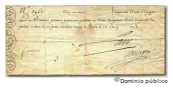
\includegraphics[width=50mm]{capitulos/img/billeteJohn} 
\label{fig:billeteJohn} 

	\footnotesize
	Figura recuperada de Wikipedia

\end{figure}

\section{La Compañía del Mississippi}
El siguiente movimiento del nuevo sistema de Law, fue la creación de la Compañía del Mississippi. Junto a esta Compañía, el banco nacional adquirió una mayor importancia.

A principios de 1.717, un conjunto de comerciantes y proveedores estaban desarrollando una gran colonia en Luisiana, que abarcaba toda la cuenca del río Mississippi. El territorio había pertenecido a Francia durante más de cuarenta años, pero hasta ahora nadie había percibido un rendimiento de él. Law se hizo cargo del proyecto con la aprobación del gobierno y lo hizo mucho más ambicioso, creando la Compañía de Occidente	\footnote{En francés: Compagnie d'Occident.} en agosto de 1.717.

La creación de la Compañía supuso la implantación de dos modelos. Uno de ellos, fue el del desarrollo de la tierra en el \emph{Nuevo Mundo}. De este modo, el gobierno entregó el territorio a la Compañía de Occidente pero sin que supusiese la pérdida de soberanía nacional, y a su vez, el gobierno esperaba beneficiarse de su desarrollo privado a través de la recaudación de impuestos. El segundo modelo a implantar, consistía en convertir deuda pública en acciones de la Compañía. Estas acciones eran potencialmente más arriesgadas, pero también más beneficiosas porque se repartía una mayor cantidad de dividendos.

Este último movimiento había supuesto un incremento de seis millones libras mientras que el valor de la Compañía se incrementó en 100 millones de libras. De hecho, la oferta de acciones comenzó el 14 de septiembre de 1.717, pero no se cerró hasta el 16 de julio de 1.718 debido al gran éxito. Una vez cerrada la operación, se tomaron medidas para acelerar el pago de la suscripción de las acciones, ya que todo el capital invertido no tenía el respaldo de las reservas de metales tales como oro y plata. Esto era debido a la emisión excesiva de billetes como moneda fiduciaria, en particular mediante la introducción de un sistema de pre-pago\footnote{Un accionista pagaba el 20 por ciento del precio y el resto lo paga en cinco meses, de lo contrario perdía el pago inicial.}. 

La suscripción se prolongó durante un largo periodo de tiempo, en parte, debido a la reclamación que los acreedores hicieron sobre el Estado, tal y como se podrá comprobar en la Figura \ref{fig:preciosAccionesIndias}. Esta reclamación, tenía su fundamento en el intercambio de bonos por acciones, ya que los intereses sobre los bonos era del 4 por ciento y fueron asignados sobre una explotación de impuestos. En julio de 1.718, la empresa propuso hacerse cargo de la explotación de tabaco beneficiándose de importantes sumas de dinero que posteriormente iban destinadas a las arcas estatales.
En un principio, el beneficio fue de cuatro millones de libras, exactamente la suma que el gobierno tendría que pagar a la empresa en concepto de intereses de los bonos de los suscriptores. Aun así, Law creía que podría funcionar mejor el monopolio esperando generar entre seis y ocho millones por año, una expectativa razonable, como se podrá comprobar a continuación.

Law se hizo cargo de los activos que provenían de Louisiana, incluyendo un barco para el que John Law contrató a personal competente y bien formado. Así, procedió a comprar, arrendar y construir nuevos buques, por lo que para diciembre de 1.718 la compañía tenía una docena de barcos a su disposición y ya se habían realizado con éxito varios viajes a Louisiana.

Al mismo tiempo, la Compañía creció debido a una serie de fusiones. Tras la concesión del monopolio del tabaco, la compañía compró otras sociedades mercantiles como la \emph{Compañía del Senegal} en diciembre de 1.718; la \emph{Compañía de las Indias}; la \emph{Compañía de China} y la \emph{Compañía de África} en junio de 1.719; la \emph{Compañía de Santo Domingo} y el monopolio de \emph{esclavos} en Guinea en Septiembre de 1.720. Esta situación concedió a la empresa el monopolio efectivo en casi todo el comercio de ultramar francés. La compañía también amplió sus actividades recaudatorias al sector agrícola en Lousiana creando los contratos de arrendamientos en julio de 1.719. Este tipo de contrato se denominó \emph{Granjas Generales} \footnote{En francés: Fermes Générales.} y en él, quedaba patente la obtención del permiso de recolecta de la mayor parte de los impuestos al consumo en Francia, a su vez, éste suponía un 30 por ciento de los ingresos del gobierno. Finalmente, a la Compañía se le concedió también el monopolio de recaudación de todos los impuestos directos\footnote{En francés: Recettes Générales.} de Francia, lo que suponía alrededor del 55 por ciento de los ingresos totales del país. En este momento, la Compañía del Mississippi pasó a denominarse como la Compañía de las Indias

Durante las primeras adquisiciones de otras compañías, la del Mississippi se fue financiando con activos iniciales de la empresa, pero la gran mayoría del resto de adquisiciones fueron financiadas con emisión de nuevas acciones. Cada nueva acción tiene igual jerarquía que las acciones antiguas, aunque la oferta aumentó con el transcurso del tiempo. La emisión inicial de fue de 200.000 acciones y se ofrecieron a 500 libras cada una, a pagar en bonos del gobierno a su valor nominal, es decir, en vez de con moneda fiduciaria, con reservas de oro o plata. En junio de 1.719 se realizó una nueva ampliación de capital de 50.000 acciones que se ofrecieron a 550 libras. En julio de 1.719 se ofertaban 50.000 acciones a 1.000 libras cada una. Y por último, en septiembre y octubre de 1.719 se amplió capital por 300.000 acciones a 5.000 libras cada una. Todas las ampliaciones de capital se debían de pagar en efectivo, es decir con reservas de oro y plata. 

De este modo, la segunda y tercera ampliación de capital, tomaron la forma de una oferta de derechos, es decir, un suscriptor de la ampliación de junio tuvo que poseer cuatro acciones originales o \emph{madres} y un suscriptor de la edición de julio tuvo que poseer cuatro acciones \emph{madres} y una acción \emph{hija} para poder comprar una acción \emph{nieta}. Este requisito provocó un mayor frenesí suscriptor  entre la población francesa.

Después de realizar el pago de las acciones, el accionista recibía un certificado por el que le daba derecho a una participación en el pago total de todo el desembolso. Esta característica, señaló Cochrane (2.001), cuando los pagos eran reembolsables, la suscripción era la primera norma. Esta función también caracterizó en la cuarta suscripción, generalmente llamada \emph{sumisión}. 


\section{La evolución de precios y el estallido de la burbuja}  
Hay que tener en cuenta dos aspectos fundamentales. El primero es que la burbuja económica no surgió espontáneamente, y el segundo, es que el nombre asignado a la burbuja en castellano no es tan revelador como el nombre en francés: \emph{Le système de Law}\footnote{En castellano podría traducirse como \emph{El sistema de Law}.}.

Sea como fuere, hay que ser conscientes de que la burbuja económica surgió gracias al manejo del mercado de John Law sobre la Compañía y sobre el propio mercado. Vale la pena señalar que, si bien la Burbuja de los Mares del Sur de Londres fue testigo de una proliferación de sistemas y empresas y un aumento sustancial en el mercado de acciones, en contraposición se encuentra la burbuja francesa que tan sólo concierne a una sola empresa \footnote{Parte del esquema de Law era comprar otras empresas comerciales, para sacarlas del mercado y obtener así el monopolio}. Law gestionaba activamente el mercado y el aumento de precios del mismo. Tal y como refleja Herbert Lüthy (1.961) en su obra: \emph{La Banque protestante en France de la rèevocation de l'Édit de Nantes á la Rèvolution}, Law había estado influyendo o manipulando el precio de las acciones de su compañía durante un largo periodo de tiempo, esto fue posible gracias a la adquisición de nuevas empresas para conseguir el monopolio.

Como desarrollo del segundo punto, cabe decir que la Compañía estaba acumulando una gran colección de Compañías rentables. El aumento de precio en las acciones de la Compañía del Mississippi refleja el hecho de que estas nuevas compañías comerciales adquiridas por Law, se convirtieron también a su vez en acciones. 

La prehistoria de la bolsa francesa no es bien conocida. En la Edad Media, los operadores de divisas en París se reunían en el llamado \emph{puente de intercambio} \footnote{En francés: Pont au Change}, cerca de la Casa de Moneda. A finales del siglo XVI los cargos oficiales fueron creados, pero no había un lugar oficial donde se reuniesen.

Cuando la compañía de Law estableció sus oficinas en la \emph{rue Quincampoix}, significó la creación de un punto local para este tipo de mercado. En ese momento el mercado se había vuelto visible. Finalmente, el gobierno decidió reconocer y regular el mercado y le dio un lugar permanente en septiembre de 1.724.

Law no sólo había creado el mercado en un sentido físico, sino que también presentó a la población francesa los tipos de instrumentos financieros conocidos por los comerciantes holandeses e ingleses. En 1.718, la suscripción de la Compañía de Occidente languidecía en el momento en el que Law anunció\footnote{Anuncio publicado en la Gaceta d'Amsterdam el 23 de mayo de 1.718.} públicamente su disposición a comprar acciones de la Compañía de Occidente a cambio de una prima del 2 por ciento. El emisor de la opción se comprometió a la entrega de una acción en cualquier momento del año siguiente en el que Law eligiese, al 70 por ciento de su valor nominal. Esta afirmación, garantizaba al accionista 100 libras en lingotes de oro del Estado, el dividendo mínimo del 4 por ciento en la participación y el porcentaje de la prima correspondiente a la ampliación de capital número dos.

Pero es en el otoño 1719, tras la conversión de la deuda y después de que la Compañía se convirtiese en un participante activo del mercado, cuando el precio de las acciones se fue mermando.

\begin{figure}[!h] 
\caption{Precios de las acciones de la Compañía de las Indias} 
\centering 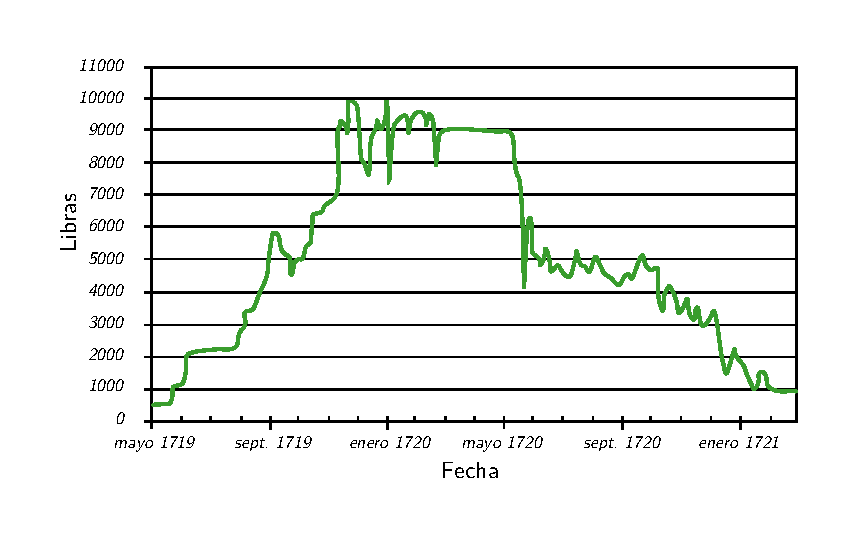
\includegraphics[width=150mm]{capitulos/graficos/preciosAccionesIndias} 
\label{fig:preciosAccionesIndias} 

	\footnotesize
	Fuente: Thornton, H (2.010)

\end{figure}

El 28 de agosto de 1.719, y tal como se puede apreciar en la Figura \ref{fig:preciosAccionesIndias}, la deuda del estado convertida en acciones, había estado avivando el precio de las acciones de 3.100 libras a 3.500 libras. Una ampliación de capital por valor de 500 millones de libras se había anunciado la noche del 14 de septiembre del mismo año, cuando los precios de las acciones se situaban en las 5.000 libras. En un plazo de tres días, las acciones ganaron otras 300 libras. Tras estas repentinas subidas de precios, éstos comenzaron a caer por en la segunda quincena de septiembre situándolo debajo de las 5.000 libras. 

A finales de octubre se tenía que efectuar el primer pago mensual, por parte de los suscriptores, correspondiente a las primeras suscripciones. Pero un decreto del 20 de septiembre consolidó los pagos mensuales en pagos trimestrales y aplazó el primero a diciembre.

La segunda ampliación de capital, se anunció el 30 de septiembre porque las acciones cayeron a 4.100 libras. El 2 de octubre, los precios alcanzaron las 4.335 libras pero al día siguiente cayeron de nuevo a 4.200 libras cuando se anunció la tercera emisión de 500 millones de libras.

El manuscrito de \emph{Giraudeau} coincide con la Figura \ref{fig:preciosAccionesIndias}, y muestra como el precio de las acciones volvió a incrementar situándose en 4.500 libras el 4 de octubre. Para los días 5 y 6 de octubre, las acciones cayeron a 3.800 libras, lo que produjo la convocatoria, por parte de Law, de una reunión con los directores de la empresa. Al día siguiente, el precio de las acciones al comienzo del día, sufrieron un aumento hasta alcanzar las 4.000 libras y se cerró en 4.250 libras. Ese mismo día, el 5 de octubre, el \emph{Banque Générale}, anunció que estaba dispuesto a comprar acciones a 4.500 libras y al día siguiente las acciones escalaron hasta esa cantidad, lo que provocó que el 7 de octubre ascendiesen a 4.750 libras.

El 13 de octubre, el banco todavía estaba comprando acciones a ese precio y el mercado se situó apenas por encima de las 4.500 libras como se puede apreciar en la Figura \ref{fig:preciosAccionesIndias}. Un real decreto del 12 de octubre, en alusión explícita a los rumores de nuevas emisiones de acciones, se comprometió formalmente a que ninguna de las otras acciones se iba a vender de manera diferente a la establecida anteriormente. A la semana siguiente, las acciones subieron a 4.900 libras.

Otro episodio de caída de precios tuvo lugar en diciembre de 1.719. El problema fue una crisis de liquidez debido a la cercanía de la fecha límite para hacer los pagos de las suscripciones. Cabe destacar que las suscripciones son opciones sobre acciones y que para mantener viva la opción, el dueño tuvo que realizar pagos periódicos. El decreto del 20 de septiembre, anteriormente mencionado, permitió que el precio de la acción se situase en 6.000 libras	\footnote{El periódico \emph{Amsterdamse Courant} irónicamente señaló que el mercado está liderado por los sucesivos decretos cual orquesta que bien podría llegar a saltarse toda una octava.}. A finales de diciembre, se debía realizar el primer pago por parte de los suscriptores, ya que no se efectuó en septiembre y la suma ascendía a 1.500 libras.

Los especuladores, tal y como se puede observar en la Figura \ref{fig:preciosAccionesIndias},  comenzaron a vender algunas suscripciones para financiar el pago de las demás, y esto llevó a la bajada de precios desde un máximo de 9.525 libras, el 2 de diciembre a 9.250 libras, el 9 de diciembre. A continuación, el 14 de diciembre, los precios se desplomaron a 7.430 libras. Del mismo modo, los derechos de suscripción cayeron de 5.700 libras el 2 de diciembre a 3.000 libras el 14 de diciembre. Ese día, el banco volvió a intervenir mediante la publicación de un precio de compra de 4.000 libras, y por la noche las suscripciones aumentaron de precio nuevamente a 4.500 libras. Sin embargo, la empresa mantiene el calendario vigente para el pago inicial de la suscripción. El siguiente rumor, fue la proximidad de la asamblea general de accionistas del 30 de diciembre. Las acciones originales llegaron a su máximo histórico el 23 de diciembre, cuando alcanzaron las 10 000 libras.

A lo largo de este período, el banco también prestó 2.500 libras al 2 por ciento anual, poniendo en peligro la seguridad del precio de la acción\footnote{La acción estaba respaldada por las reservas de oro y plata.}. Este hecho,  provocó una bajada en el precio de la acción y fomentó la especulación con el incentivo del \emph{dinero fácil}. La cantidad de dinero prestada ascendió a 276 millones de libras.

El 30 de diciembre de 1.719, en la Asamblea General, se decidió abrir una oficina en la que las acciones y las suscripciones pudieran ser compradas y vendidas para los precios publicados cada día. Esta oficina funcionó de manera intermitente, cerrándose ente entre el 10 y el 15 de enero, y abriendo sus puertas de nuevo a partir del 29 enero y hasta el 10 febrero. Por último, el precio de las acciones el 5 de marzo, se fijaron en 9.000 libras. En mayo de 1.720, la empresa había comprado 800 millones de libras en acciones, alrededor del 16 por ciento de su capitalización, con adición de emisión de moneda fiduciaria.

A partir de enero de 1.720, ya no se pudo considerar el precio de las acciones como \emph{precio de mercado}. El mercado se puede controlar si no existen manipuladores, pero como ya se ha mencionado, la manipulación del mercado por parte de Law, era una característica crucial de este sistema financiero con el fin de que el precio de las acciones siguiese al alza. En agosto de 1.719, la conversión de la adquisición de las compañías comerciales en acciones fue una catástrofe a largo plazo para la Compañía del Mississippi y para el gobierno, dando lugar así, a un precio ficticio de las acciones.

La manipulación del sistema tuvo consecuencias desastrosas para John Law, ya que probablemente se dio cuenta de que existían grandes incoherencias y trató de subsanarlas desarrollando una serie de políticas financieras entre finales de febrero y principios de marzo de 1.720. 

El 22 de febrero de 1.720, La \emph{Banque Générale} se fusionó con la Compañía con la intención de impedir crédito a la Corona. El efecto sobre los precios fue inmediato como se puede comprobar en la Figura \ref{fig:preciosAccionesIndias}. De 9.425 libras el 22 de febrero a 8.000 libras el 1 de marzo, mientras que el precio las suscripciones se redujo de 6.600 libras a 5.450 libras. La reacción de Law fue inmediata ya que retrocedió unos pasos en cuanto al precio de las acciones se refiere. El 5 de marzo, se abrió otra oficina para la compra y venta de acciones a un precio fijo de 9.000 libras. Al mismo tiempo, las suscripciones pendientes perdieron sus opciones y fueron convertidas en acciones a una proporción de 2 por 3, mientras que los reembolsos de la deuda pública se siguieron realizando, pero en billetes del banco. Desde marzo hasta finales de mayo de 1.720, la compañía pasó otros 1.319,5 millones de libras a dinero papel para comprar el 28 por ciento de sus acciones, lo que supone un aumento colosal en cuanto al valor de la compañía.

El desastre ya se estaba gestando. Law fue obligado por el Consejo del Rey a controlar la oferta monetaria nominal, bien reduciendo un gran número de billetes en circulación o mediante la reducción del nominal de cada billete. Como se puede observar en la Figura \ref{fig:preciosAccionesIndias}, el 21 de mayo de 1.720, la confianza de los compradores llegó a su fin provocando el estallido de la burbuja económica. Entre junio y agosto de 1.720, se tuvieron que recomprar los billetes y las acciones con la moneda antigua. Realizándose así el 15 de agosto, una desmonetización gradual de los billetes. En noviembre de 1.720, el experimento monetario de John Law había finalizado y la compañía de Law era declarada insolvente. Law fue al exilio el 18 de diciembre.

Con la siguiente Figura \ref{fig:ComparaMississippiMaresSur}, se va poder observar los precios alcanazados por la Compañía del Mississippi y por la COmpañía de los Mares del Sur, explicada en el capítulo que viene a continuación.

\begin{figure}[!h] 
\caption{Comparación de precios de las acciones entre la Compaía del Mississippi y la Compañía de los Mares del Sur} 
\centering 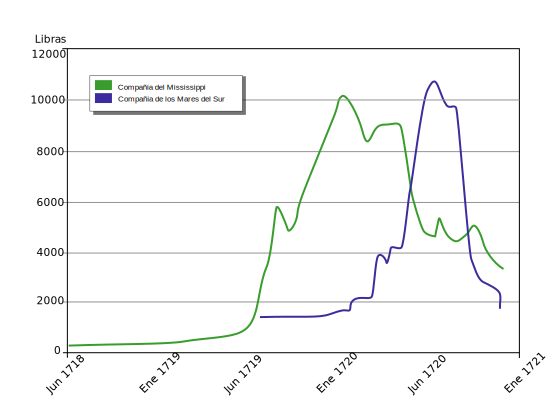
\includegraphics[width=150mm]{capitulos/graficos/ComparaMississippiMaresSur} 
\label{fig:preciosAccionesIndias} 

	\footnotesize
	Fuente: William Goetzman (2.010)

\end{figure}
